\documentclass[border=10pt]{standalone}

\usepackage{tikz}
\usepackage{tikzsymbols}
\usetikzlibrary{calc,patterns,shapes.geometric}

\def\centerarc[#1](#2)(#3:#4:#5){\draw[#1] ($(#2)+({#5*cos(#3)},{#5*sin(#3)})$) arc (#3:#4:#5);}

\begin{document}
	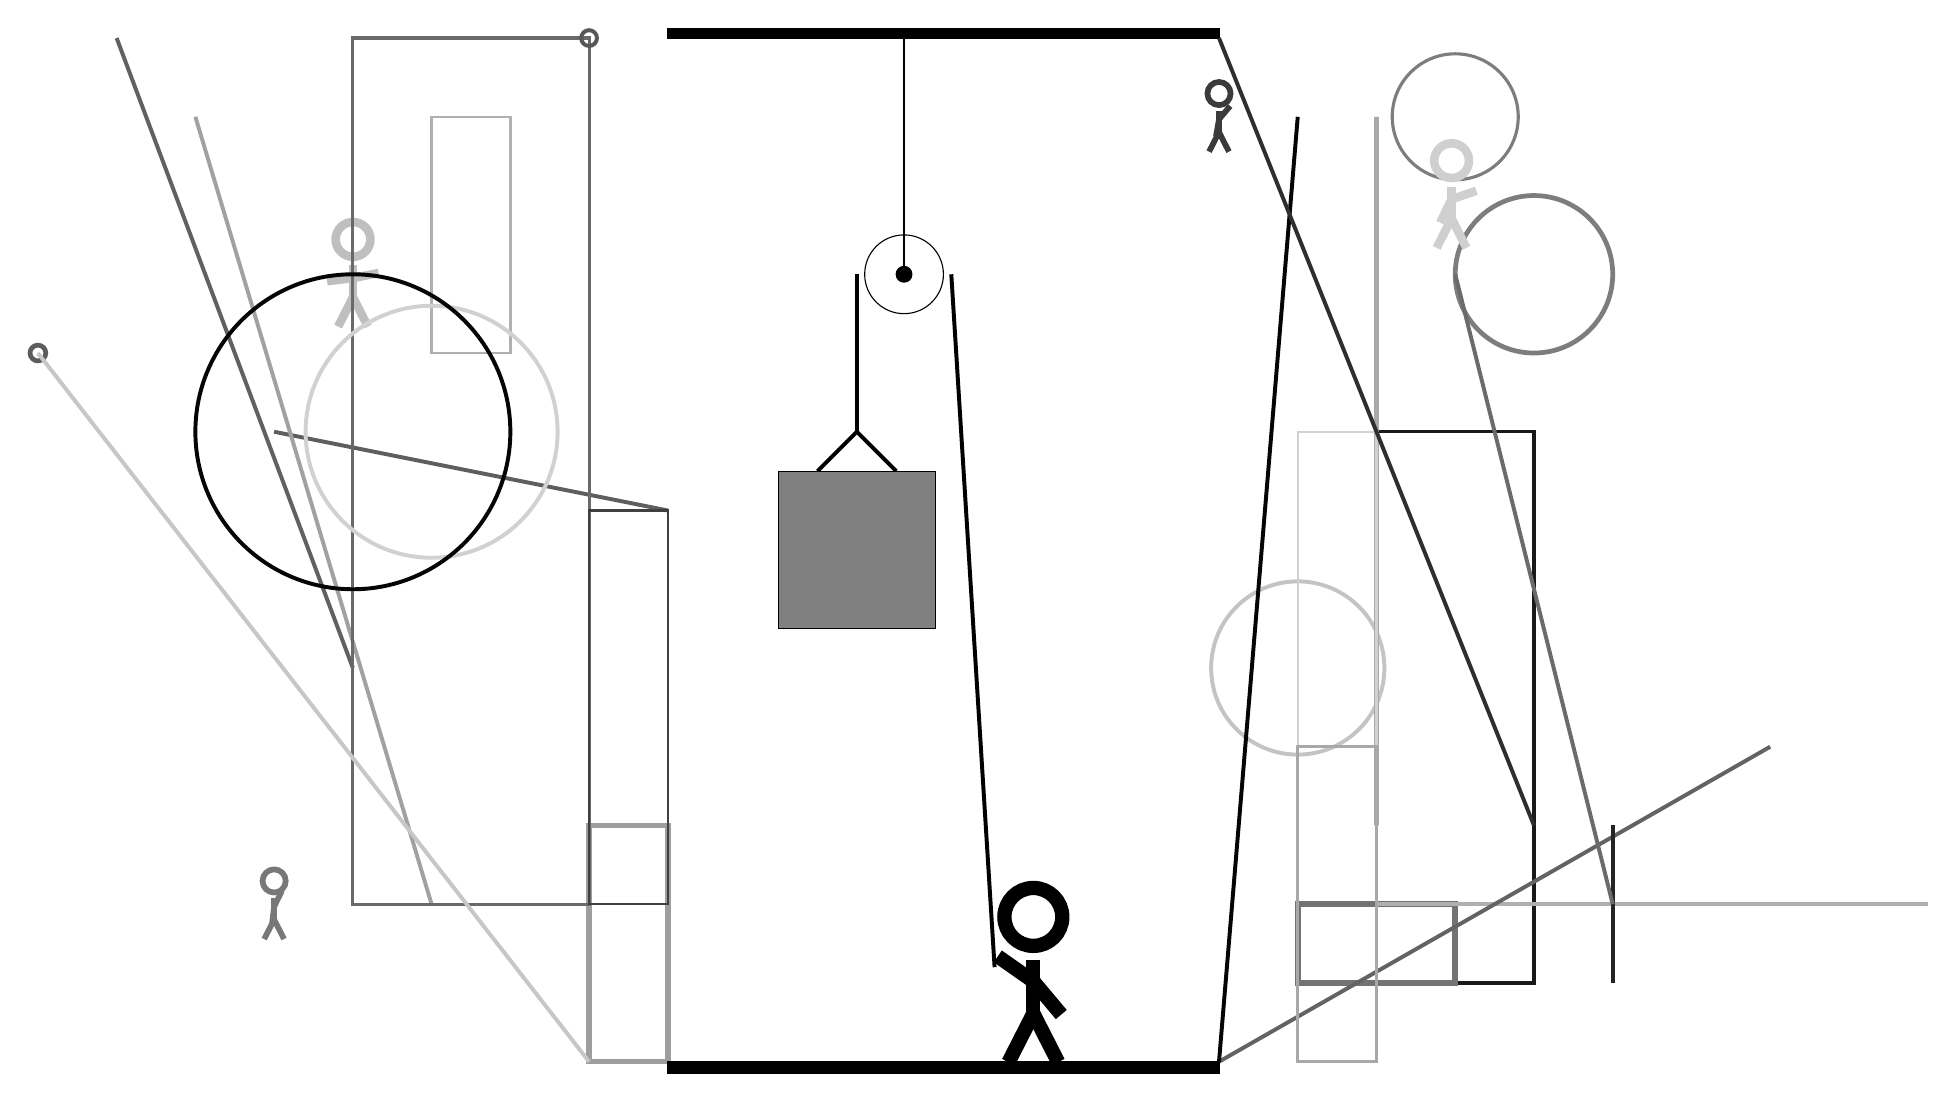
\begin{tikzpicture}
		%%%%% START %%%%%
		
		\draw[fill=black] (-2, 10) rectangle (5, 10.125);
		
		\draw (1, 7) circle (0.5);
		\draw[fill=black] (1, 7) circle (0.1);
		\draw (1, 10) -- (1, 7);
		
		\draw[line width=0.5mm] (-0.1, 4.5) -- (0.4, 5.0) -- (0.9, 4.5);
		\draw[fill=black!50] (-0.6, 4.5) rectangle (1.4, 2.5);
		
		\draw[line width=0.5mm] (0.4, 7) -- (0.4, 5.0);
		\centerarc[line width=0.5mm](1, 7)(0:180:0.6);
		\draw[line width=0.5mm](1.6, 7) -- (2.15, -1.8);
		
		\node at (2.6, -1.9) {\Strichmaxerl[10][-35][-50]};
		
		\draw[line width=0.4mm, color=black!90] (7, 5) rectangle (9, -2);
		
		\node[line width=0.7mm, color=black!53] at (-7, -1) {\Strichmaxerl[4][83][64]};
		\draw[line width=0.5mm, color=black!62](-6, 2) -- (-9, 10);
		\draw [line width=0.6mm, color=black!23](14, 9) circle (0.0);
		\draw[line width=0.7mm, color=black!55] (6, -2) rectangle (8, -1);
		\node[line width=0.6mm, color=black!77] at (5, 9) {\Strichmaxerl[4][80][50]};
		\node[line width=0.4mm, color=black!25] at (-6, 7) {\Strichmaxerl[6][7][11]};
		\draw[line width=0.5mm, color=black!63](-7, 5) -- (-2, 4);
		\draw[line width=0.7mm, color=black!38] (-3, -3) rectangle (-2, 0);
		\draw[line width=0.5mm, color=black!37](-5, -1) -- (-8, 9);
		\draw[line width=0.4mm, color=black!59] (-3, 10) rectangle (-6, -1);
		\draw [line width=0.5mm, color=black!23](6, 2) circle (1.1);
		\draw[line width=0.7mm, color=black!34] (7, 9) rectangle (7, 0);
		\draw[line width=0.5mm, color=black!31](7, -1) -- (14, -1);
		\draw[line width=0.3mm, color=black!31] (-4, 9) rectangle (-5, 6);
		\draw [line width=0.6mm, color=black!64](-10, 6) circle (0.1);
		
		\draw[line width=0.3mm, color=black!18] (7, 5) rectangle (6, -3);
		\draw[line width=0.5mm, color=black!22](-3, -3) -- (-10, 6);
		\draw[line width=0.5mm, color=black!61](5, -3) -- (12, 1);
		\draw [line width=0.5mm, color=black!18](-5, 5) circle (1.6);
		\draw [line width=0.5mm, color=black!66](-3, 10) circle (0.1);
		
		\draw [line width=0.6mm, color=black!51](9, 7) circle (1.0);
		\draw [line width=0.5mm, color=black!98](-6, 5) circle (2.0);
		\draw [line width=0.4mm, color=black!51](8, 9) circle (0.8);
		\draw[line width=0.4mm, color=black!34] (7, -3) rectangle (6, 1);
		
		\node[line width=0.6mm, color=black!19] at (8, 8) {\Strichmaxerl[6][64][19]};
		\draw[line width=0.5mm, color=black!98](6, 9) -- (5, -3);
		\draw[line width=0.5mm, color=black!82](9, 0) -- (5, 10);
		
		\draw[line width=0.5mm, color=black!86](10, -2) -- (10, 0);
		\draw[line width=0.5mm, color=black!58](10, -1) -- (8, 7);
		\draw[line width=0.3mm, color=black!75] (-3, 4) rectangle (-2, -1);
		
		
		\draw[fill=black] (-2, -3) rectangle (5, -3.15);
		
		%%%%% END %%%%%
	\end{tikzpicture}
\end{document}